\section{Auswertung}
\label{sec:auswertung}

\subsection{Eichung der Messanlage}
Für die Eichung der Messanlagen wurden Messungen der Frequenzspektren von verschiedenen Ketten aus Zylinderresonatoren aufgenommen. Die Messung wurde sowohl mit dem Oszilloskop als auch mit dem Computer aufgenommen. Die Ergenisse sind in der 
Abbildung \ref{fig:zyl1-6-12} dargestellt. 
\begin{figure}[H]
    \centering
    \begin{tabular}{cc}
      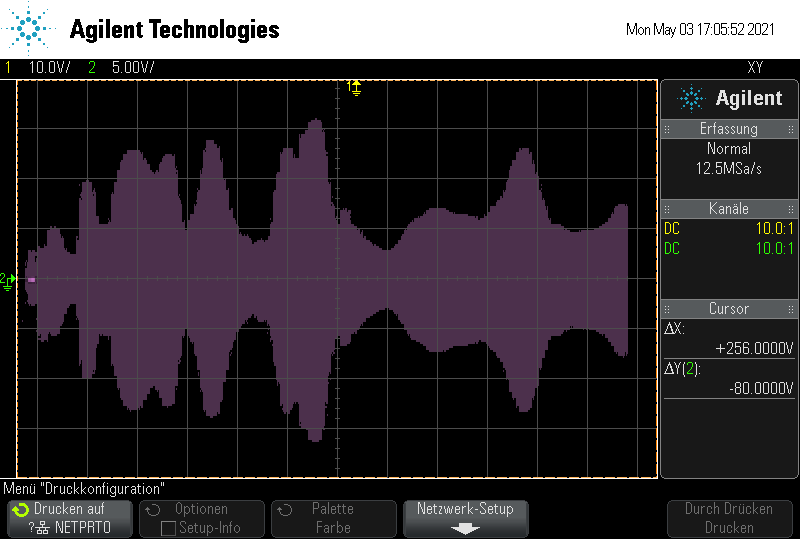
\includegraphics[width=65mm]{Daten/Zyinder/Zylinder_1.png} &   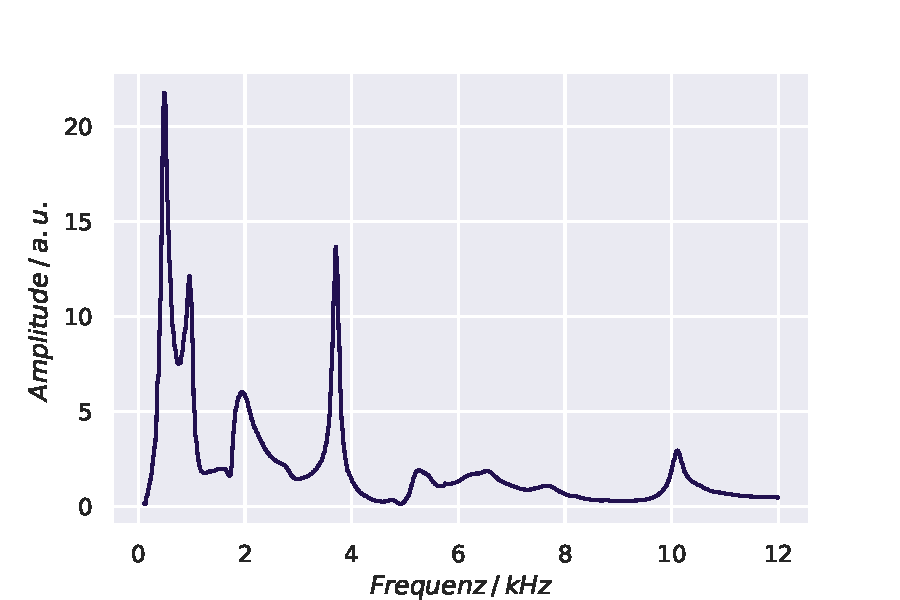
\includegraphics[width=65mm]{Daten/Zyinder/Zylinder_1.pdf} \\
    (a) 1 Zylinder & (b) 1 Zylinder \\[6pt]
     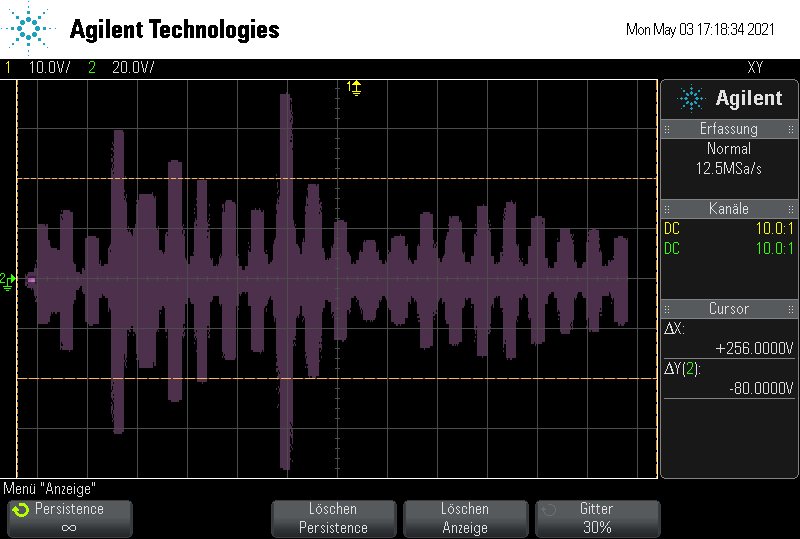
\includegraphics[width=65mm]{Daten/Zyinder/Zylinder_6.png} &   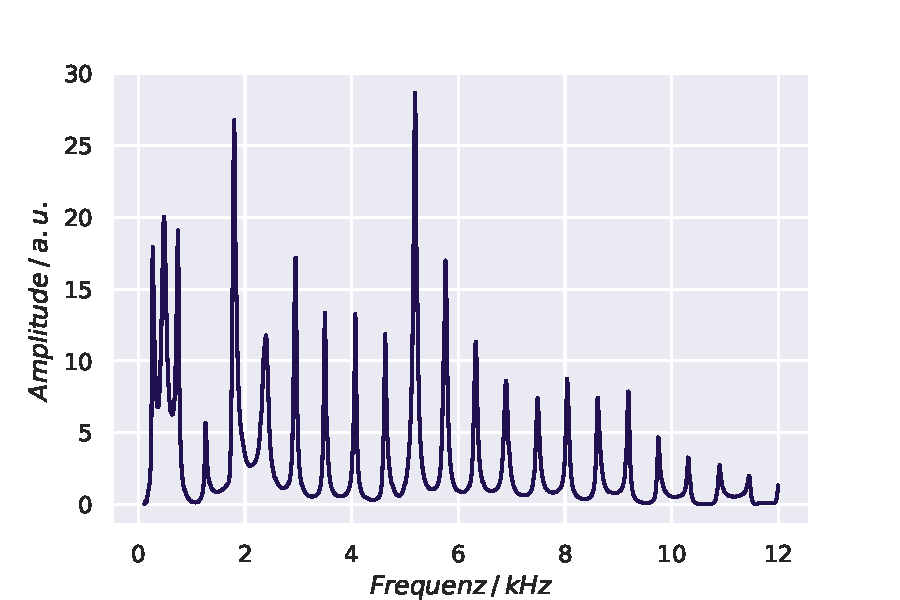
\includegraphics[width=65mm]{Daten/Zyinder/Zylinder_6.pdf} \\
    (c) 6 Zylinder & (d) 6 Zylinder \\[6pt]
    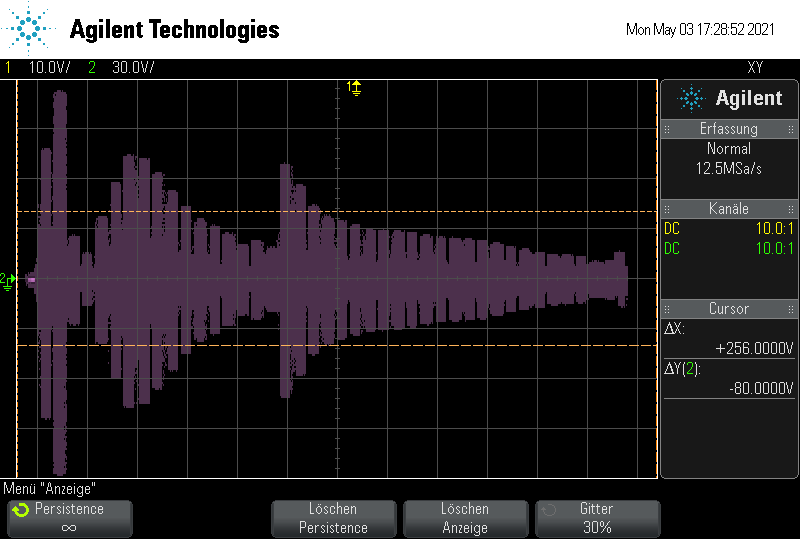
\includegraphics[width=65mm]{Daten/Zyinder/Zylinder_12.png} &   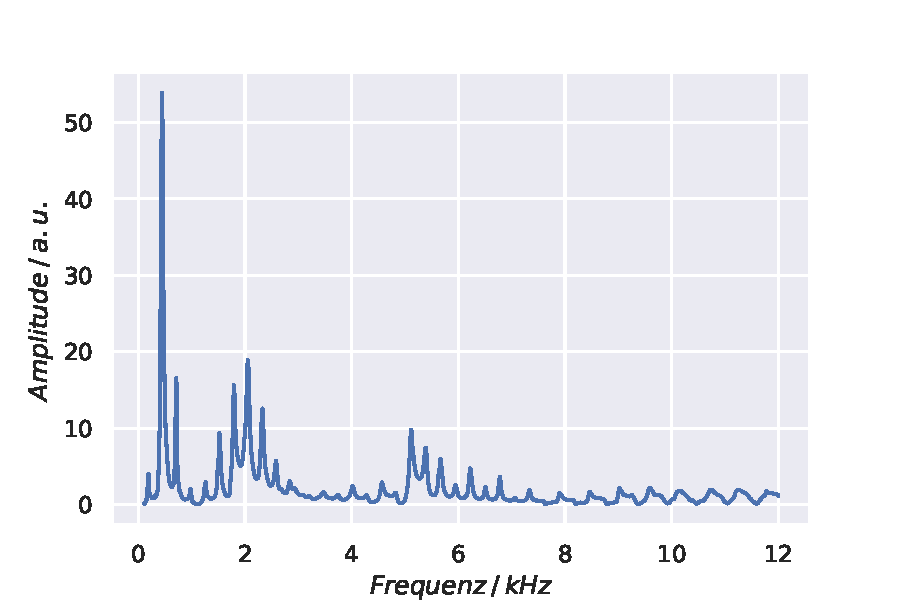
\includegraphics[width=65mm]{Daten/Zyinder/Zylinder_12.pdf} \\
    (c) 12 Zylinder & (d) 12 Zylinder \\[6pt]
    \end{tabular}
    \caption{Gemessene Frequenzspektren der Zylinder-Resonatoren mit unterschiedlicher Länge. Die Messung am Oszillator ist links angegeben und die Messung am Computer rechts. } 
    \label{fig:zyl1-6-12}
\end{figure}

Die Messungen mit dem Oszilloskop zeigen den selben Verlauf wie die Messungen mit dem Computer. Es ist bei allen Messungen das charakteristische Spektrum eines Festkörpers ersichtlich. Die einzelnen Peaks geben die Resonanzen wieder der Zylinderkette. Wie erwartet, nimmt auch die Amplitude mit steigender Frequenz ab. 
Somit bestätigen die Messungen insgesamt die Erwartungen und die Eichung war damit erfolgreich. 
Es ist zu erwähnen, dass die Messung des einzelnen Zylinders ersichtlich nur unsauber gelungen ist. Hier sind die Resonanzen des Zylinders nicht eindeutig erkennbar. Für die weiteren Messungen sind jedoch scharfe Peaks an den Resonanzfrequenzen zu erkennen. \\
Hieran anschließend, wurde das Spektrum eines Zylinders der Länge $75\,\si{\milli\metre}$ aufgenommen. Das Spektrum ist in der Abbildung \ref{fig:fkp75mm} zu sehen.

\begin{figure}[H]
    \centering
    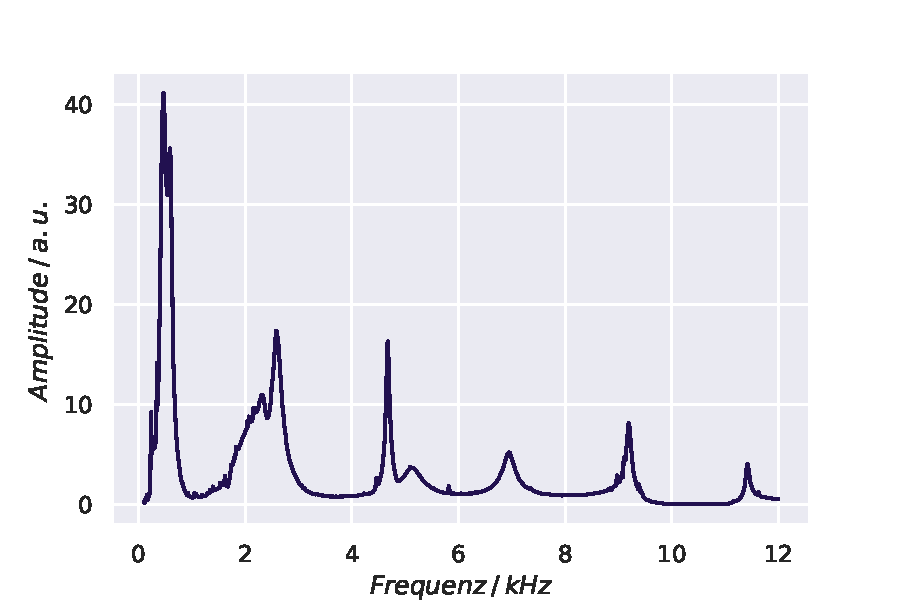
\includegraphics[width=0.8\textwidth]{Daten/Festkörper/FK_75mm.pdf}
    \caption{Das Frequenzspektrum eines $75 \,\si{\milli\metre}$ langen Zylinder-Resonators. }
    \label{fig:fkp75mm}
\end{figure}
An diesem Spektrum sind periodisch auftretende Resonanzen ersichtlich. Die Resonanzen des $75 \,\si{\milli\metre}$ Zylinders müssen an den Frequenzen auftreten, die ca. $\frac{2}{3}$ der Resonanzfrequenzen des $50 \,\si{\milli\metre}$ Zylinders entsprechen. 
Dies folgt aus der größeren Länge des Zylidners. Die stehende Welle des $75 \,\si{\milli\metre}$ Zylinders hat die $1.5$-fache Wellenlänge der stehenden Welle des $50 \,\si{\milli\metre}$ Zylinders. Die Frequenz ist umgekehrt proportional zur Wellenlänge und damit folgt der Faktor $\frac{2}{3}$.

\subsection{Das Wasserstoffatom}
Das Frequenzspektrum des Kugelresonators bei einer Ausrichtung von $\theta = 180°$ wurde mit dem Computer aufgenommen und in der Abbildung \ref{fig:h180} grafisch dargestellt. 
Die beschrifteten Resonanzen werden in der folgenden Analyse für die Berechnung der Druckamplitude verwendet. 
\begin{figure}[H]
    \centering
    \begin{tabular}{c}
    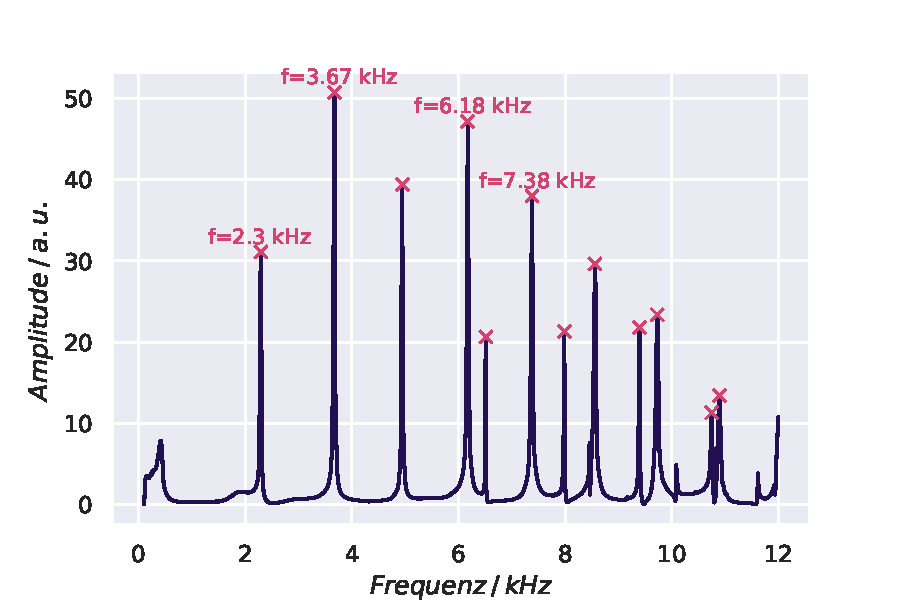
\includegraphics[width=0.9\textwidth]{Daten/Wasserstoff/H_180.pdf} \\
    (a) Messung am Computer \\[6pt]
    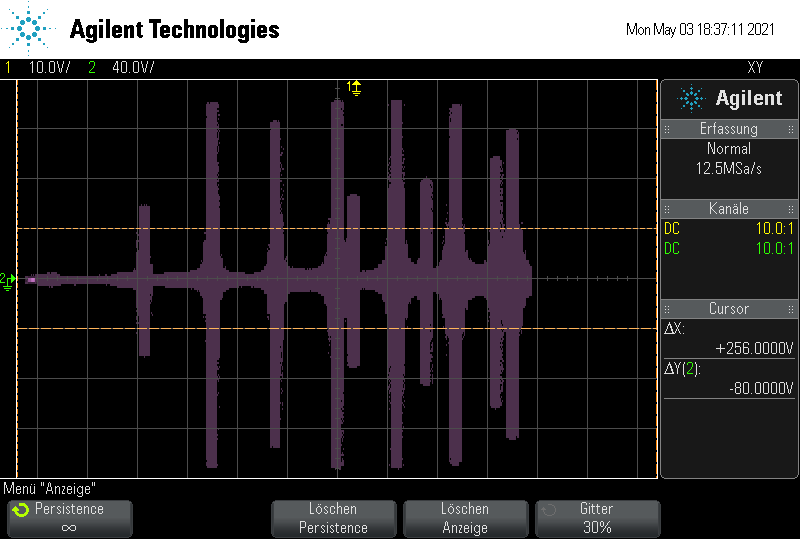
\includegraphics[width=0.9\textwidth]{Daten/Wasserstoff/H_180.png} \\
    (b) Messung am Oszilloskop \\[6pt]
    \end{tabular}
    \caption{Das Frequenzspektrum eines kugelförmigen Hohlraumresonators bei einer Ausrichtung von $\theta = 180\si{°}$ in dem Bereich $0.1 \,\si{\kilo\hertz}$ bis $10 \,\si{\kilo\hertz}$. }
    \label{fig:h180}
\end{figure}

\subsubsection{Druckamplitude}
Für die Berechnung der Druckamplitude mithilfe der gemessenen Werte wird der Ausrichtungswinkel $\theta$ folgendermaßen in den Polarwinkel $\varphi$ umgerechnet:
\begin{align*}
  \varphi = \arccos(\frac{1}{2} \cos(\theta) - \frac{1}{2}).
\end{align*}
Diese Umrechnung folgt aus einer Analyse mit Drehmatrizen \cite{qa-dresden}. Die in Abbildung \ref{fig:h180} beschrifteten Resonanzfrequenzen (also $2.3 \,\si{\hertz}$, $3.67 \,\si{\hertz}$, $6.18 \,\si{\hertz}$ und $7.38 \,\si{\hertz}$) werden nur in Abhängigkeit der Auslenkung in $10°$-Schritten erneut gemessen. 
Die Messung wird in Abhängigkeit des Polarwinkels in Abbildung \ref{fig:hpeaks} aufgetragen. In der selben Abbildung befindet sich der theoretisch erwartete Verlauf bzw. die entsprechenden Legendrepolynome. 
\begin{figure}[H]
  \centering
  \begin{tabular}{cc}
    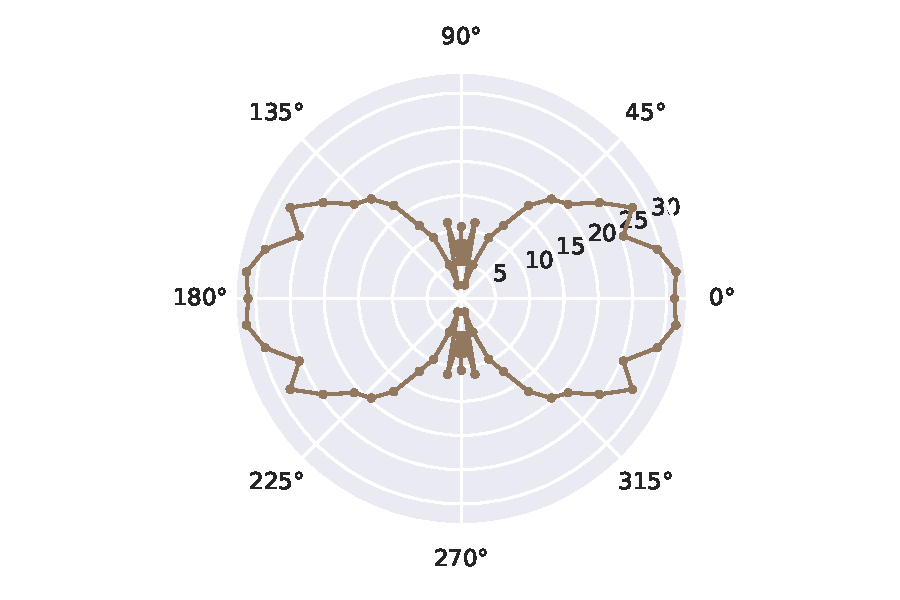
\includegraphics[width=0.5\textwidth]{Daten/Wasserstoff/peak0.pdf} &   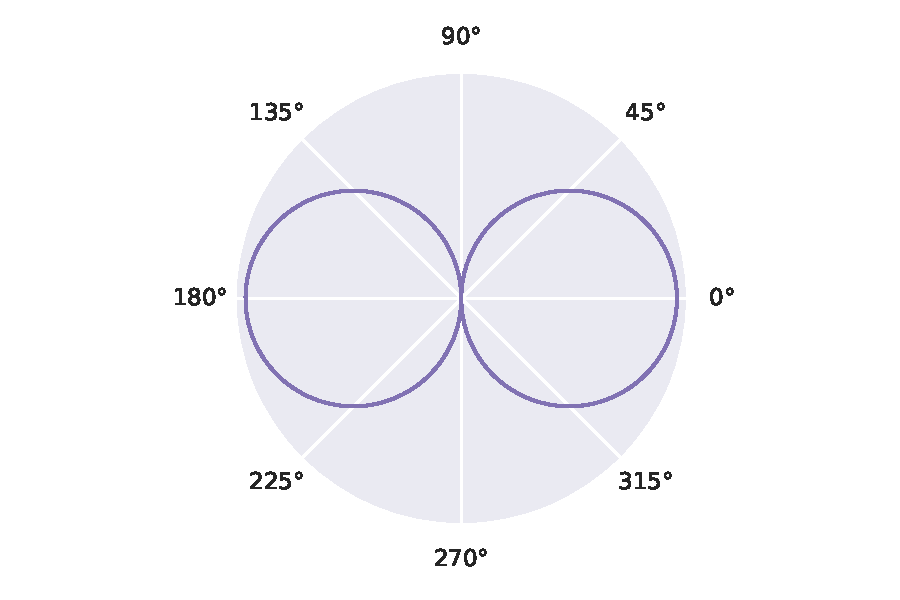
\includegraphics[width=0.5\textwidth]{Daten/Wasserstoff/peakLeg0.pdf} \\
  (a) Resonanz bei $2.3 \,\si{\kilo\hertz} $& (b) $P_1(\cos(\phi))$ \\[6pt]
  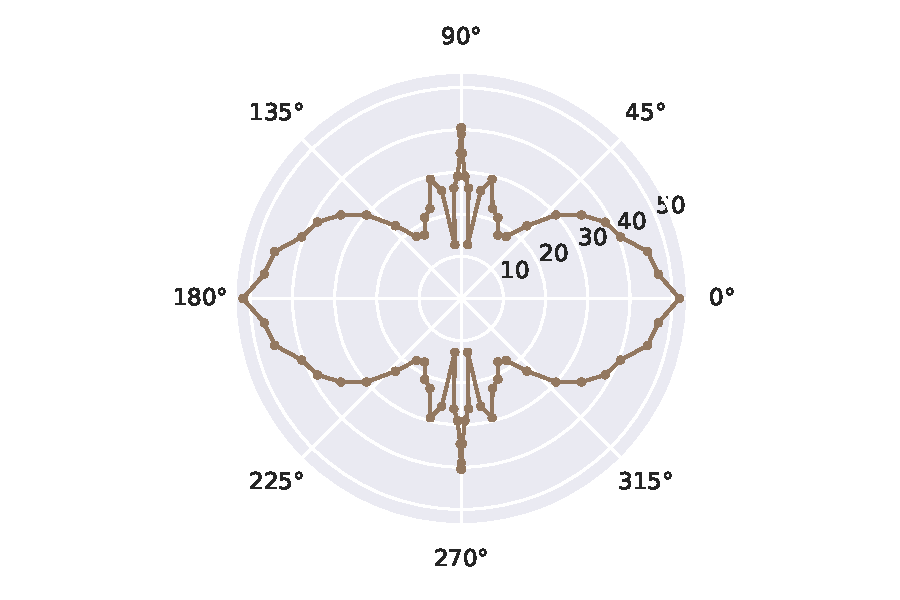
\includegraphics[width=0.5\textwidth]{Daten/Wasserstoff/peak1.pdf} &   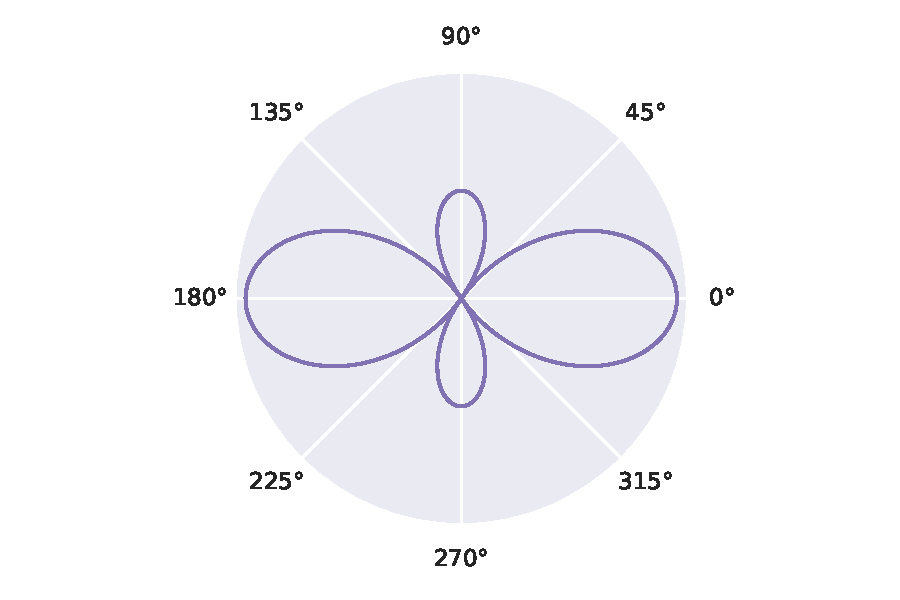
\includegraphics[width=0.5\textwidth]{Daten/Wasserstoff/peakLeg1.pdf} \\
  (c) Resonanz bei $3.67 \,\si{\kilo\hertz}$ & (d) $P_2(\cos(\phi))$ \\[6pt]
  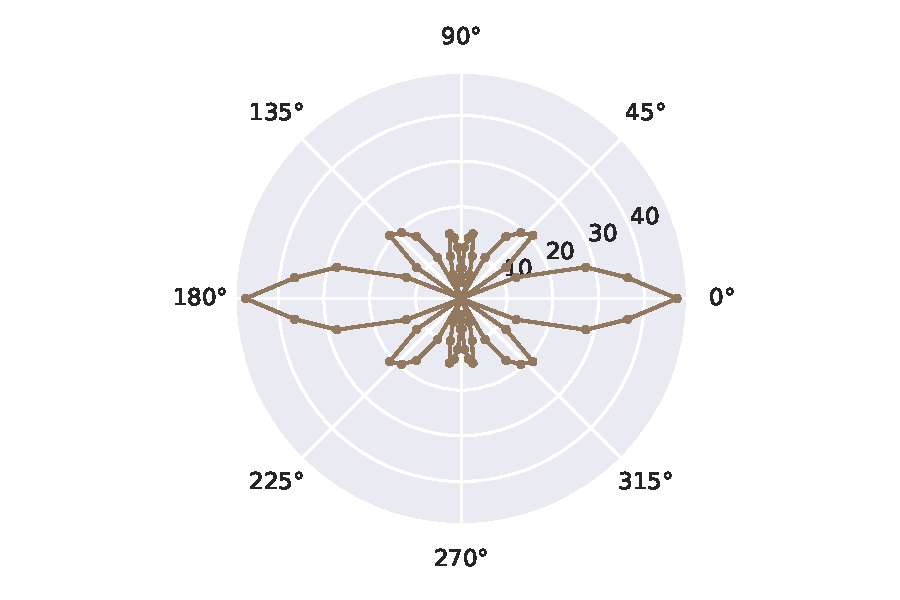
\includegraphics[width=0.5\textwidth]{Daten/Wasserstoff/peak2.pdf} &   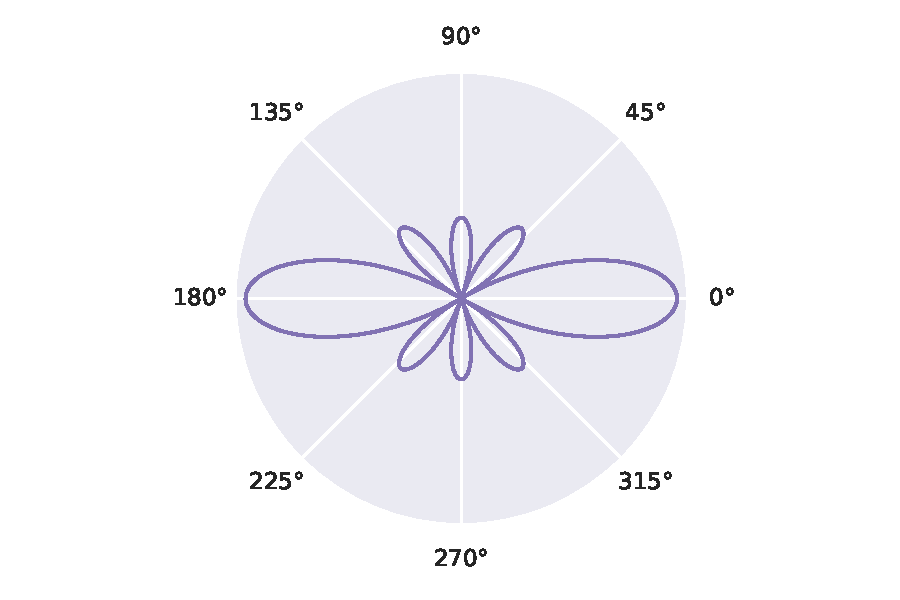
\includegraphics[width=0.5\textwidth]{Daten/Wasserstoff/peakLeg2.pdf} \\
  (c) Resonanz bei $6.18 \,\si{\kilo\hertz}$ & (d) $P_4(\cos(\phi))$ \\[6pt]
  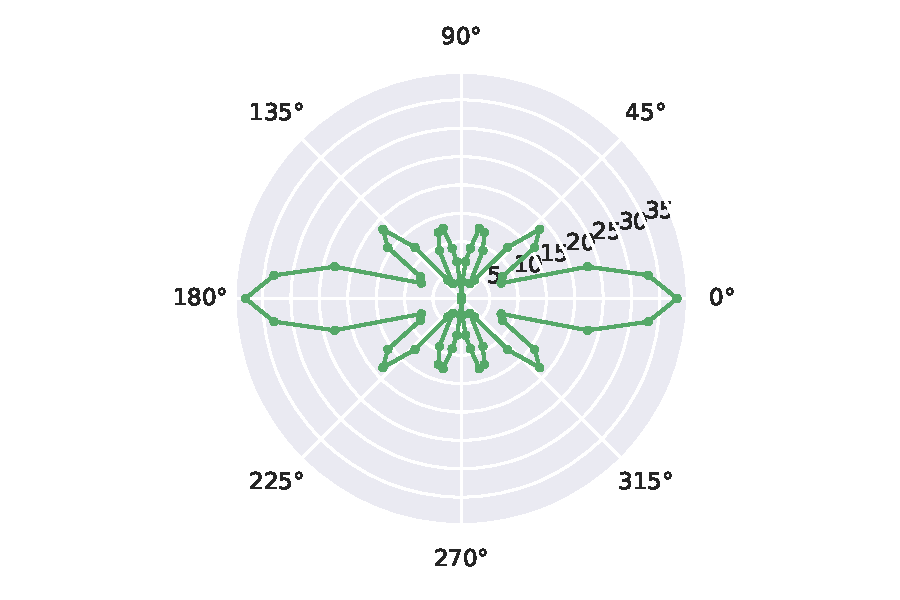
\includegraphics[width=0.5\textwidth]{Daten/Wasserstoff/peak3.pdf} &   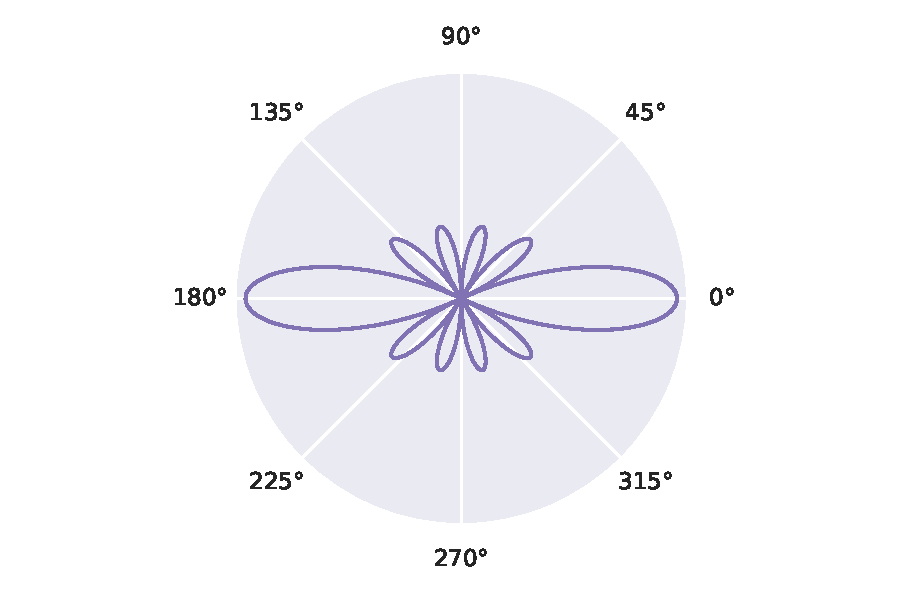
\includegraphics[width=0.5\textwidth]{Daten/Wasserstoff/peakLeg3.pdf} \\
  (c) Resonanz bei $7.38 \,\si{\kilo\hertz}$ & (d) $P_5(\cos(\phi))$ \\[6pt]
  
  \end{tabular}
  \caption{Amplitudenmessung an den Resonanzfrequenzen in Abhängigkeit vom Azimutwinkel $\phi$ neben der passenden Legendrepolynome. } 
  \label{fig:hpeaks}
\end{figure}
\subsubsection{Aufspaltung der Peaks}
In diesem Abschnitt werden die Frequenzspektren um die Resonanz bei $2.3 \,\si{\kilo\hertz}$ bei einer Ausrichtung von $\theta = 0°$ aufgenommen mit Blenden verschiedener Dicke aufgenommen. Das Ergebnis sind in den Abbildungen \ref{fig:hspalt} dargestellt. 
Die Resonanz spaltet sich in zwei Peaks auf, da die Kugelsymmetrie des Resonators durch die Blenden gebrochen wird. Der Abstand der Peaks ist ungefähr proportional zur Dicke der Blenden.
\begin{figure}[H]
  \centering
  \begin{tabular}{cc}
    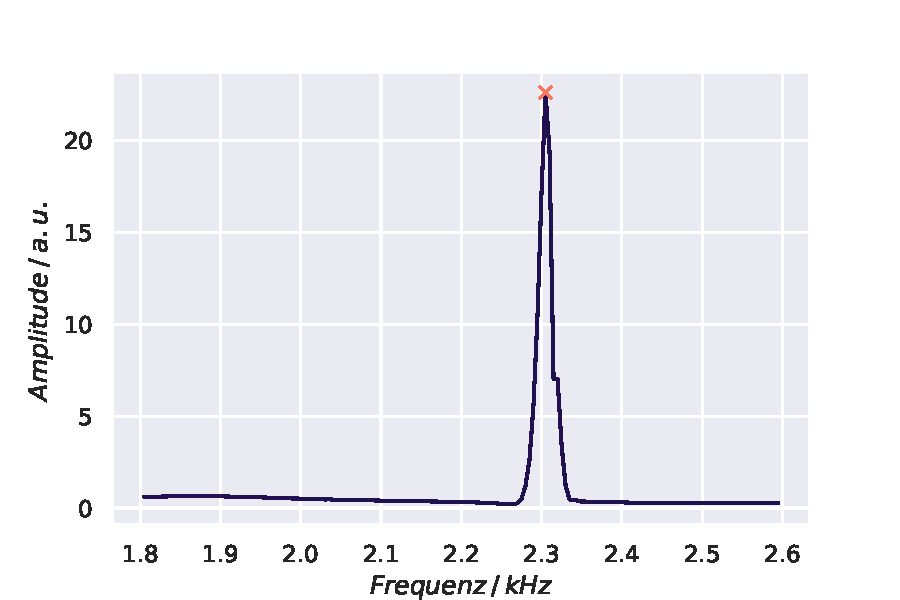
\includegraphics[width=0.5\textwidth]{Daten/Wasserstoff/spalt0.pdf} &   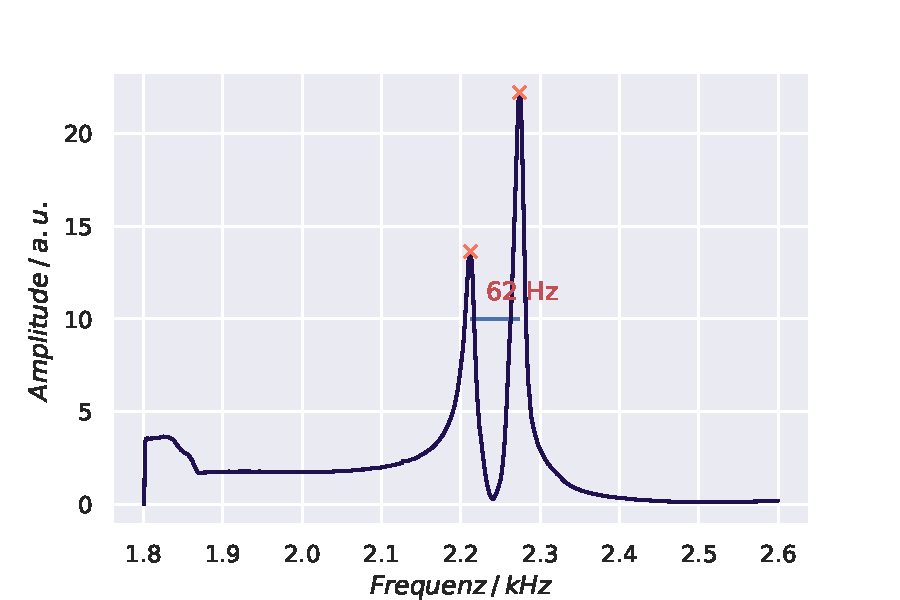
\includegraphics[width=0.5\textwidth]{Daten/Wasserstoff/spalt1.pdf} \\
  (a) Ohne Ring & (b) $3 \,\si{\milli\metre}$ Ring \\[6pt]
  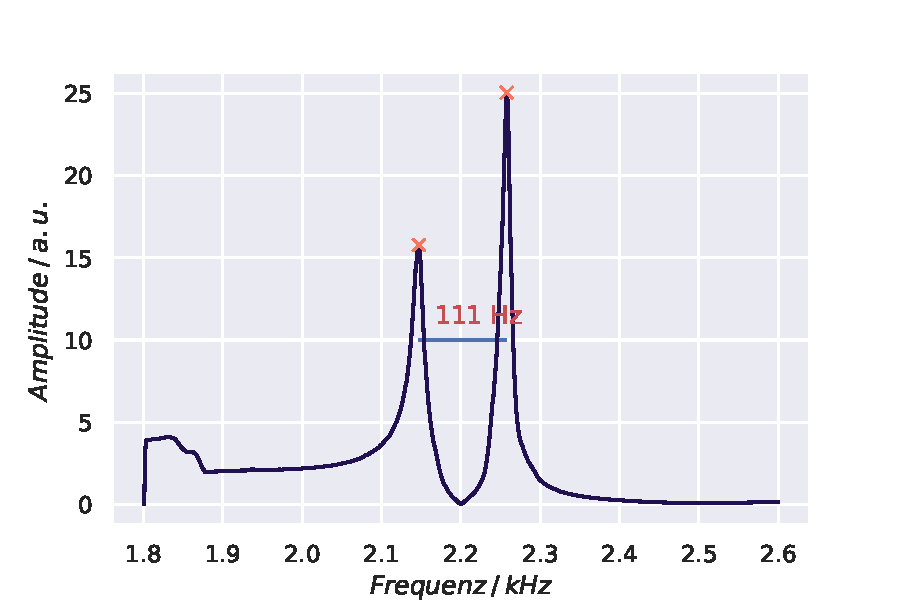
\includegraphics[width=0.5\textwidth]{Daten/Wasserstoff/spalt2.pdf} &   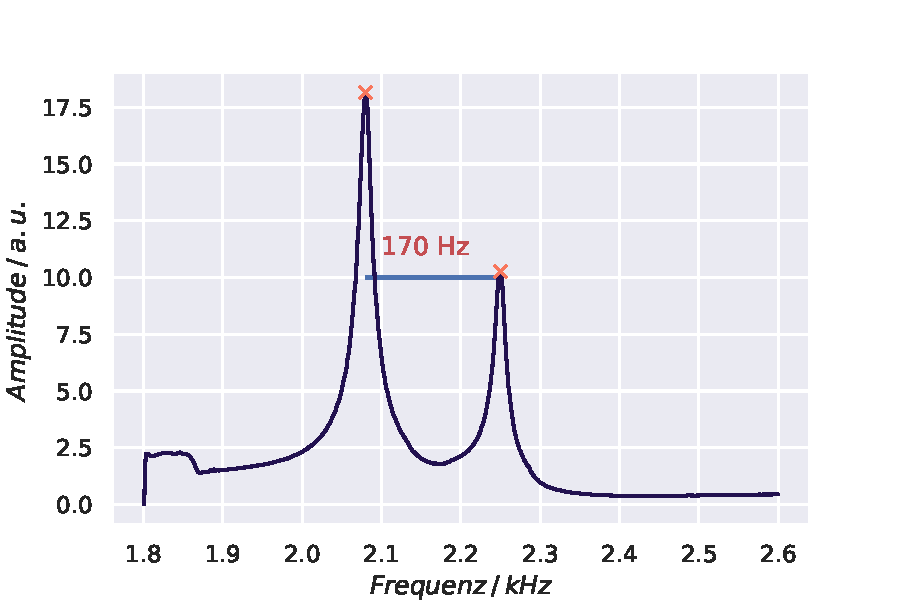
\includegraphics[width=0.5\textwidth]{Daten/Wasserstoff/spalt3.pdf} \\
  (c)  $6 \,\si{\milli\metre}$ Ring & (d)  $9 \,\si{\milli\metre}$ Ring \\[6pt]
  \multicolumn{2}{c}{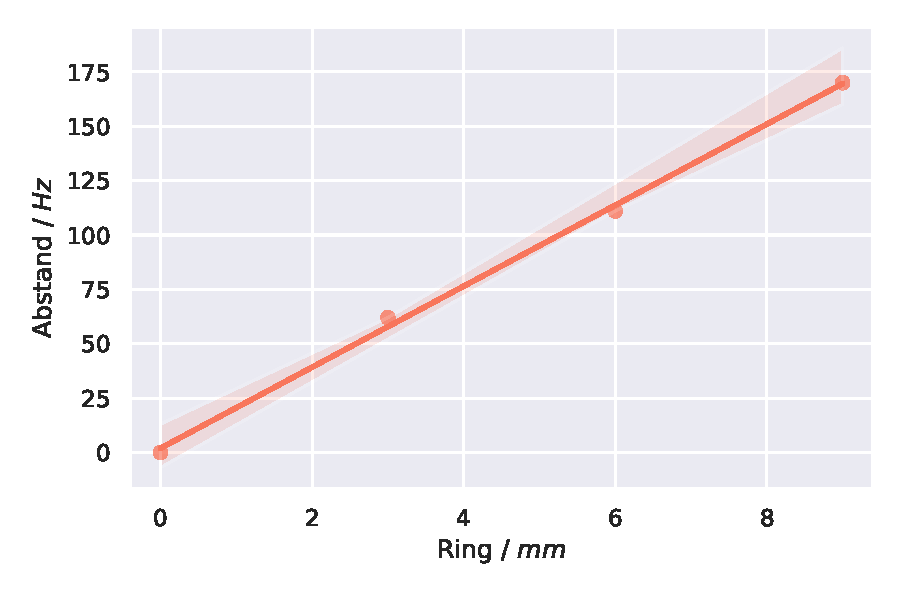
\includegraphics[width=0.65\textwidth]{Daten/Wasserstoff/spaltGesamt.pdf}}\\[6pt]
  \multicolumn{2}{c}{(e) Abstand in Abhängigkeit von der Blendendicke.}
  \end{tabular}
  \caption{Aufspaltung des Peaks bei $2.3 \,\si{\kilo\hertz}$ nachdem verschiedene Ringe die Kugelsymmetrie brechen.} 
  \label{fig:hspalt}
\end{figure}
\subsubsection{Druckamplitude mit der $9 \,\si{\milli\metre}$ Blende}
Die Druckamplitude wurde um die Frequenz $2.25 \,\si{\kilo\hertz}$ und in der Abbildung \ref{fig:9mm} aufgezeichnet. Die zugehörigen Legendrepolynome sind ebenfalls in der Abbildung zu sehen. Der Vergleich liefert die Quantenzahlen 
$l = 2 $ und $m=0$. Es ergibt sich das $3D$-Orbital eines Wasserstoffatoms.
\begin{figure}[H]
  \centering
  \begin{tabular}{cc}
    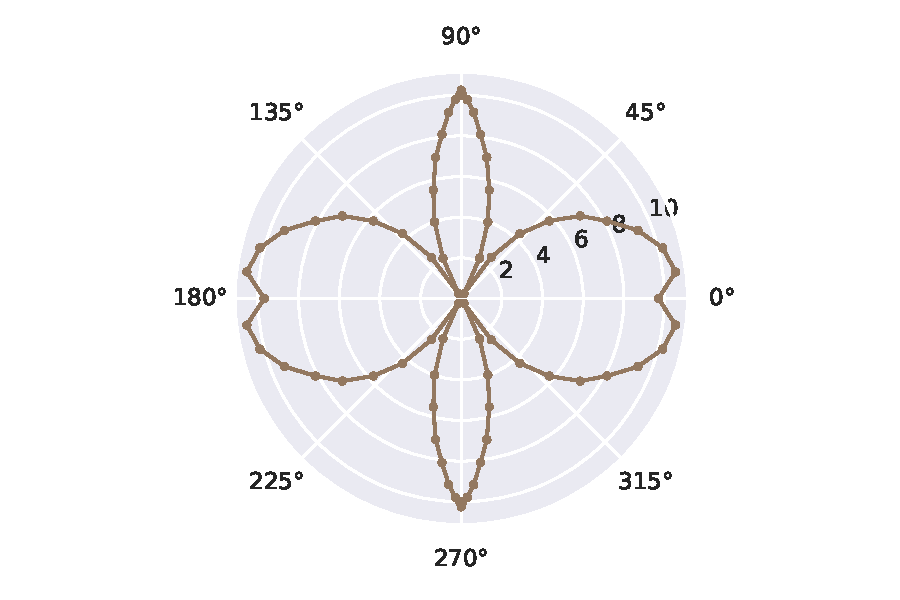
\includegraphics[width=0.5\textwidth]{Daten/Wasserstoff/peak9mm.pdf} &   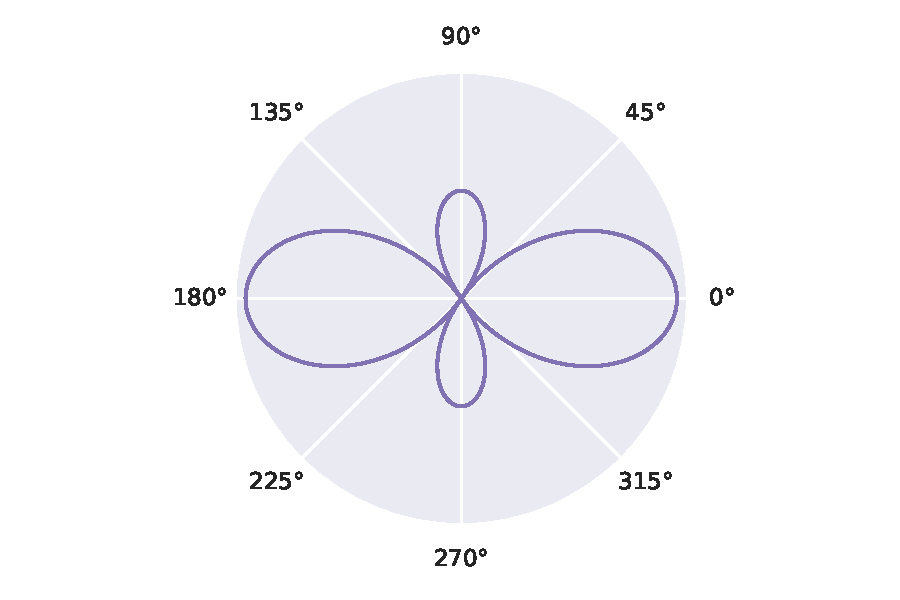
\includegraphics[width=0.5\textwidth]{Daten/Wasserstoff/peakLeg1.pdf} \\
  (a) Gemessene Druckamplitude & (b) $P_2(\cos(\phi))$ \\[6pt]
  \end{tabular}
  \caption{Gemessene Druckamplitude der $2.25 \,\si{\kilo\hertz}$ Resonanz mit der $9 \,\si{\milli\metre}$ Blende mit den zugehörigen Legendrepolynomen.} 
  \label{fig:9mm}
\end{figure}
\subsection{Das Wasserstoffmolekül}
\subsubsection{Änderung des Frequenzspektrums in Abhängigkeit des Blendendurchmessers}
\label{sec:h2peaks}
Ein Wasserstoffmolekülion ist anhand zwei gekoppelter Kugelresonatoren modelliert. Die folgenden Messungen wurden mit Blenden verschiedener Durchmesser zwischen den Kugelresonatoren 
aufgenommen. Das Frequenzspektrum dieses gekoppelten Resonators wurde für die Blenden mit $5\,mm$, $10\,mm$, $15\,mm$ und $20\,mm$ Durchmesser gemessen und in der Abbildung \ref{fig:h2} visualisiert. \\\\

\begin{figure}[H]
  \centering
  \begin{tabular}{cc}
    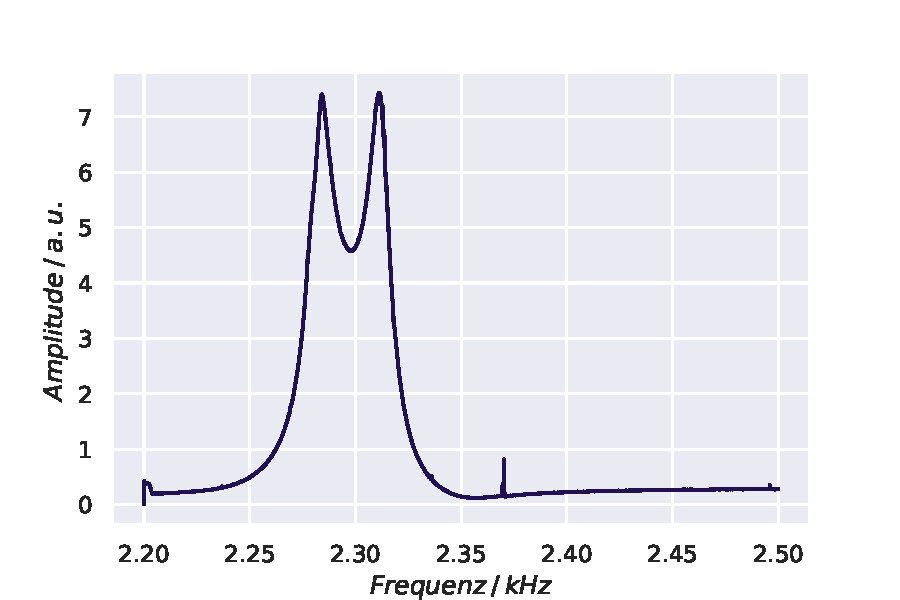
\includegraphics[width=0.5\textwidth]{Daten/Wasserstoffmolekuelion/H2_5mm.pdf} &   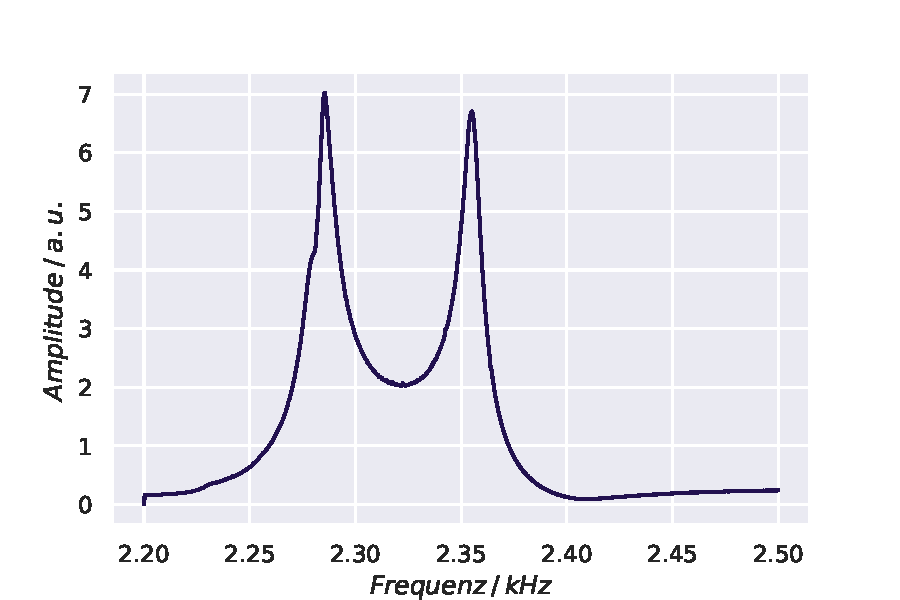
\includegraphics[width=0.5\textwidth]{Daten/Wasserstoffmolekuelion/H2_10mm.pdf} \\
  (a) $5 \, \si{\milli\metre}$  & (b) $10 \, \si{\milli\metre}$ \\[6pt]
  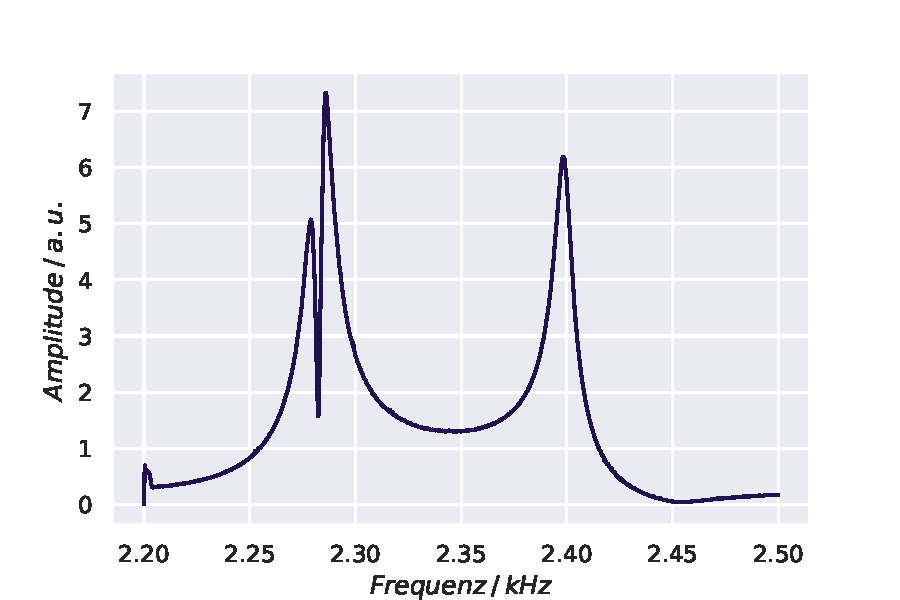
\includegraphics[width=0.5\textwidth]{Daten/Wasserstoffmolekuelion/H2_15mm.pdf} &   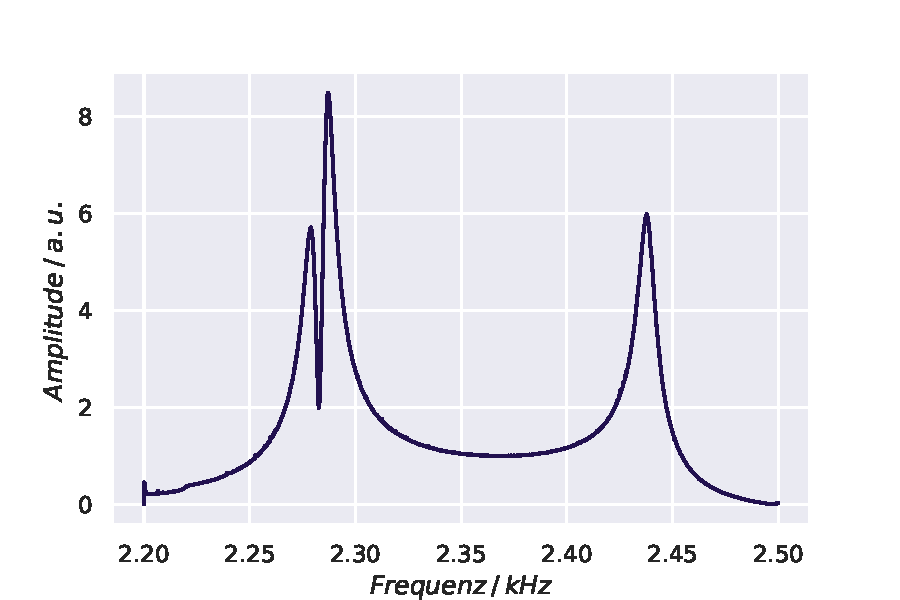
\includegraphics[width=0.5\textwidth]{Daten/Wasserstoffmolekuelion/H2_20mm_180.pdf} \\
  (c)  $15 \, \si{\milli\metre}$ & (d)  $20 \, \si{\milli\metre}$ \\[6pt]
  \multicolumn{2}{c}{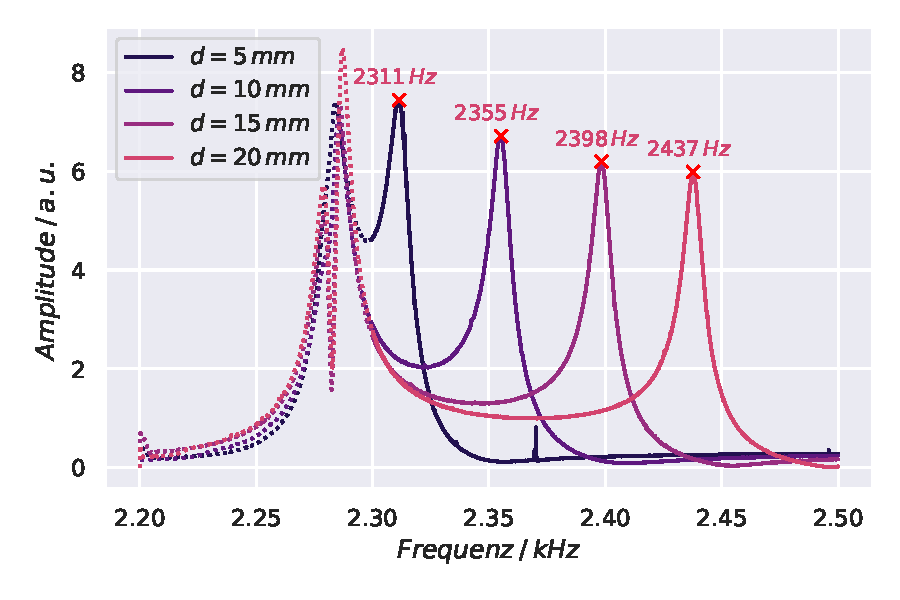
\includegraphics[width=0.65\textwidth]{Daten/Wasserstoffmolekuelion/blendAbhaeng.pdf}}\\[6pt]
  \multicolumn{2}{c}{(e) Vergleich}
  \end{tabular}
  \caption{Frequenzspektren des gekoppelten Resonators in Abhängigkeit der verschiedenen Blendendurchmesser.} 
  \label{fig:h2}
\end{figure}
\begin{figure}[H]
  \centering
  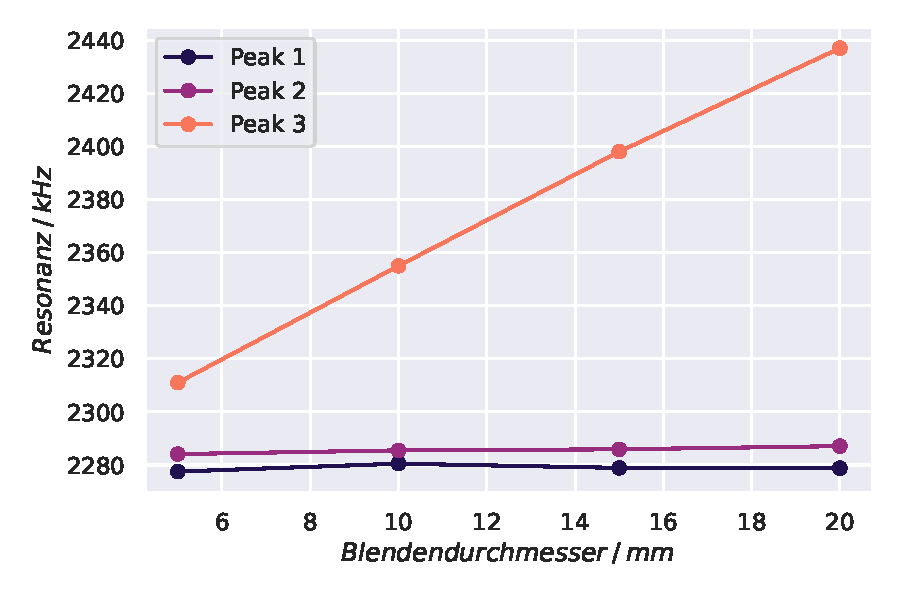
\includegraphics[width=0.8\textwidth]{Daten/Wasserstoffmolekuelion/resonanzBlend.pdf}
  \caption{Resonanzfrequenzen des gekoppelten Resonators in Abhängigkeit der verschiedenen Blendendurchmesser}
  \label{fig:h2Res}
\end{figure}
\subsubsection{Winkelverteilung mit der $20 \, mm$ Blende}
Die Winkelverteilung der drei Peaks aus Abschnitt \ref{sec:h2peaks} wurden in $10°$ Schritten aufgenommen und in der Abbildung \ref{fig:h2_2} wiedergegeben. \\
Die Verteilungen der ersten beiden Peaks weisen keine erkennbare Struktur auf und können aus diesem Grund nicht identifiziert werden.  Die Verteilung des dritten Peak jedoch 
deckt exakt die Form der Legendrepolynomen $P_0(\cos(\phi))$. Damit liegt nahe, dass der dritte Peak den anti-bindenden Zustand mit $m=1$ zeigt.  
\begin{figure}[H]
  \centering
  \begin{tabular}{cc}
  \multicolumn{2}{c}{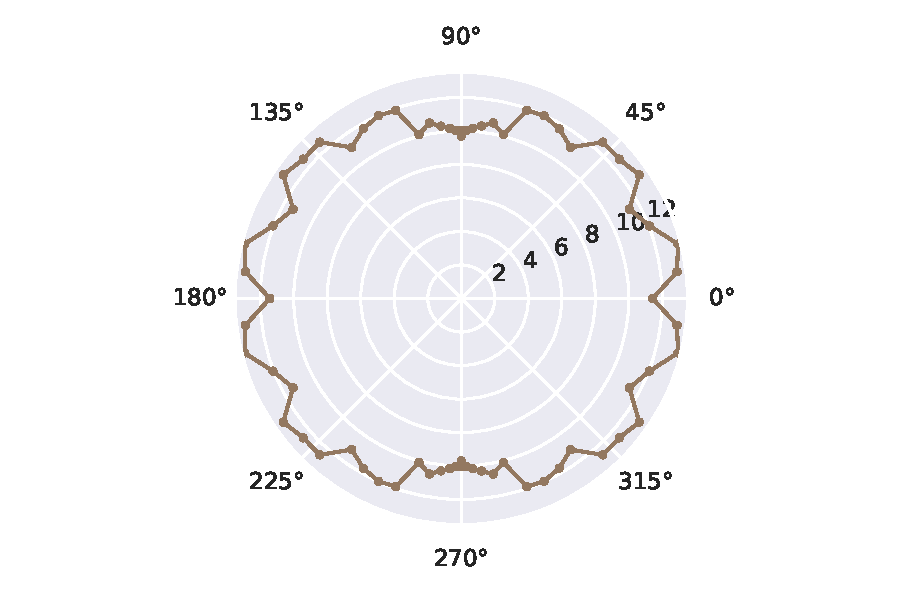
\includegraphics[width=0.5\textwidth]{Daten/Wasserstoffmolekuelion/peak0.pdf}}\\[6pt]
  \multicolumn{2}{c}{(a) Peak 1}\\[6pt]
  \multicolumn{2}{c}{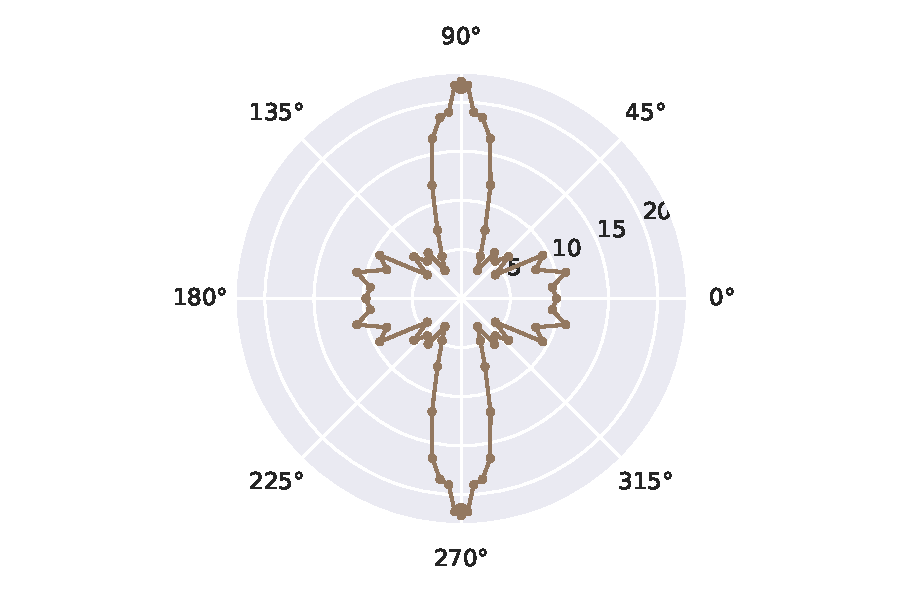
\includegraphics[width=0.5\textwidth]{Daten/Wasserstoffmolekuelion/peak1.pdf}}\\[6pt]
  \multicolumn{2}{c}{(b) Peak 2}\\[6pt]
  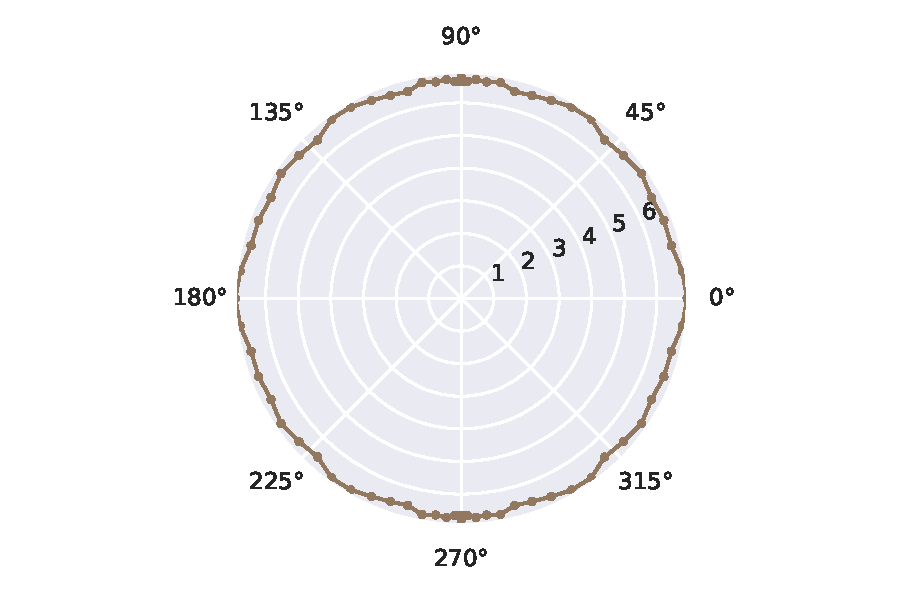
\includegraphics[width=0.5\textwidth]{Daten/Wasserstoffmolekuelion/peak2.pdf} &   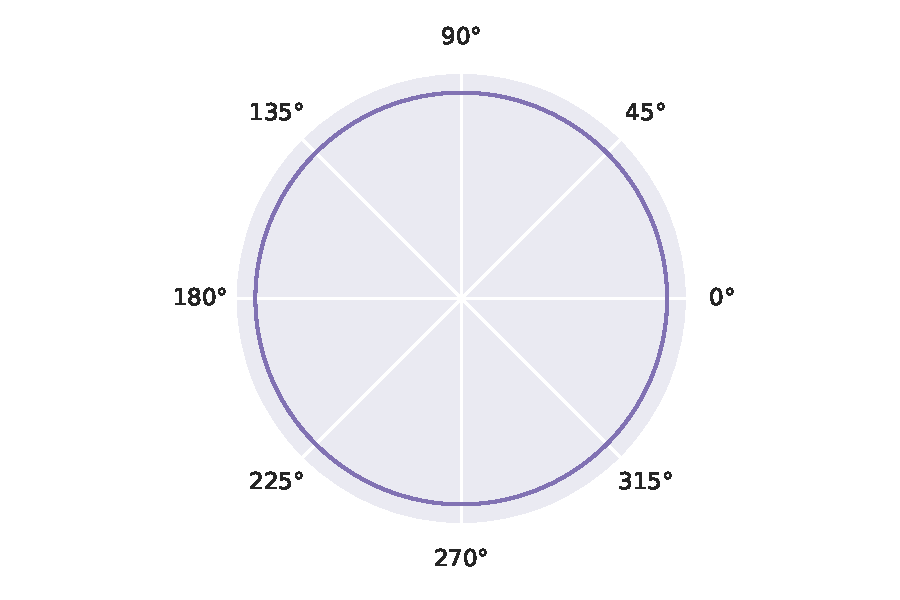
\includegraphics[width=0.5\textwidth]{Daten/Wasserstoffmolekuelion/peakLeg.pdf}\\[6pt]
  (c)  Peak 3 & (d)  $P_0(\cos(\phi))$ \\[6pt]
  \end{tabular}
  \caption{Winkelverteilung des gekoppelten Resonators bei einem Blendendurchmesser von $20\, mm$ mit passenden Legendrepolynomen.} 
  \label{fig:h2_2}
\end{figure}
\subsection{Zylinderketten als Modell für eindimensionale Festkörper}
\subsubsection{Der Übergung von einem Molekül zum Festkörper}
In diesem Abschnitt wurden die Frequenzspektren von Zylinderketten mit einer wachsenden Anzahl an Zylindern gemessen. Die Ergebnisse für Ketten mit $2$,$4$,$6$ und $10$ Zylindern und einem Blendendurchmesser von $16\, mm$ sind in der 
Abbildung \ref{fig:fk1} angegeben.\\
In der Festkörperphysik beschreiben Bänder die dicht beieinander liegende Resonanzfrequenzen der Elektronen in einem Festkörper. Diese entsprechen den Schwingungen welche sich nur wenig von den Eigenschwingungen der anderen Elektronen unterscheiden. 
In dem betrachteten Modell werden diese Schwinungen durch Schallwellen dargestellt. In der Abbildung \ref{fig:fk1} sind deutlich Bänder zu erkennen, welche auch unabhängig von der Anzahl der Zylinder sind. 
Die Bänder selbst werden durch verschiedene stehende Schallwellen im Zylinder erzeugt. Die stehende Welle kann beschrieben werden durch 
\begin{align*}
  \Psi(x) = A\cdot \sin(k_x x),  & \:\:k_x = \frac{2 \pi n_x}{L}
\end{align*}
wobei $A$ die Amplitude angibt und $n_x \in \mathbb{N}$ ist. Das $L$ gibt die Länge der Zylinder an. \\
Die Abbildung \ref{fig:fk1} zeigt, dass die Amplitude der Resonanzfrequenzen mit steigender Frequenz abnimmt. Dies kann damit erklärt werden, dass höhere Frequenzen höhere Energien benötigen. Damit sinkt die Amplitude aufgrund der Energieerhaltung. 

\begin{figure}[H]
  \centering
  \begin{tabular}{cc}
    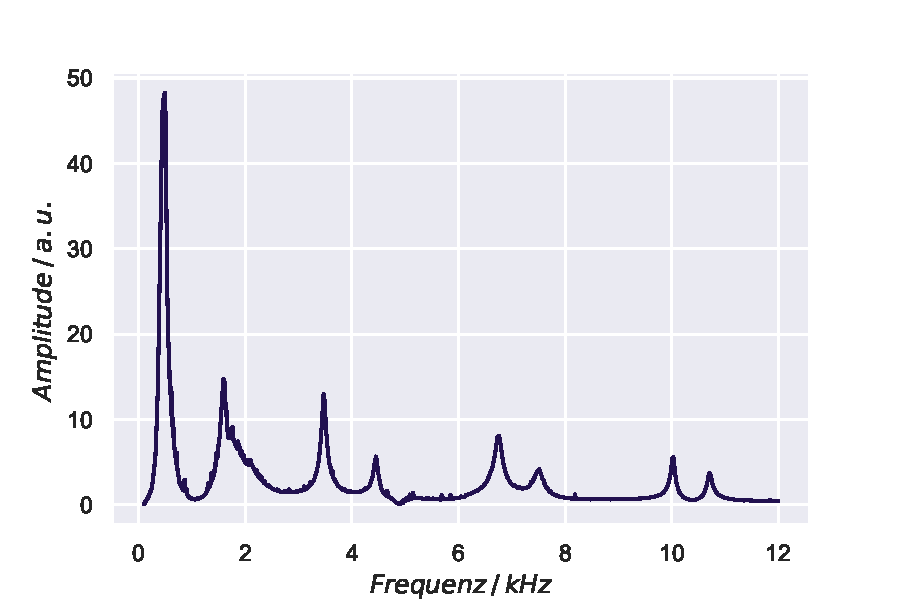
\includegraphics[width=0.5\textwidth]{Daten/Festkörper/FK1_16mm_1.pdf} &   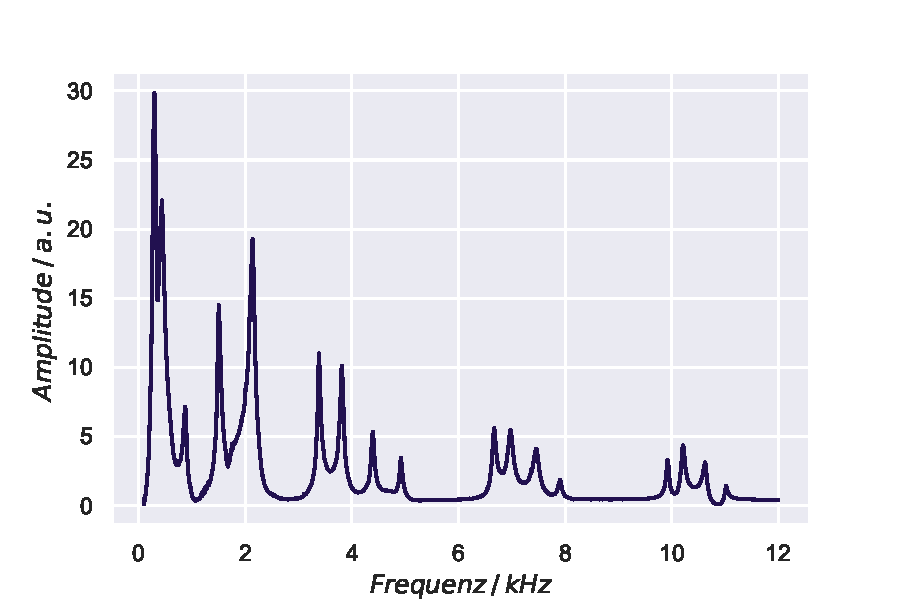
\includegraphics[width=0.5\textwidth]{Daten/Festkörper/FK1_16mm_3.pdf} \\
  (a) 2 Zylinder & (b) 4 Zylinder \\[6pt]
  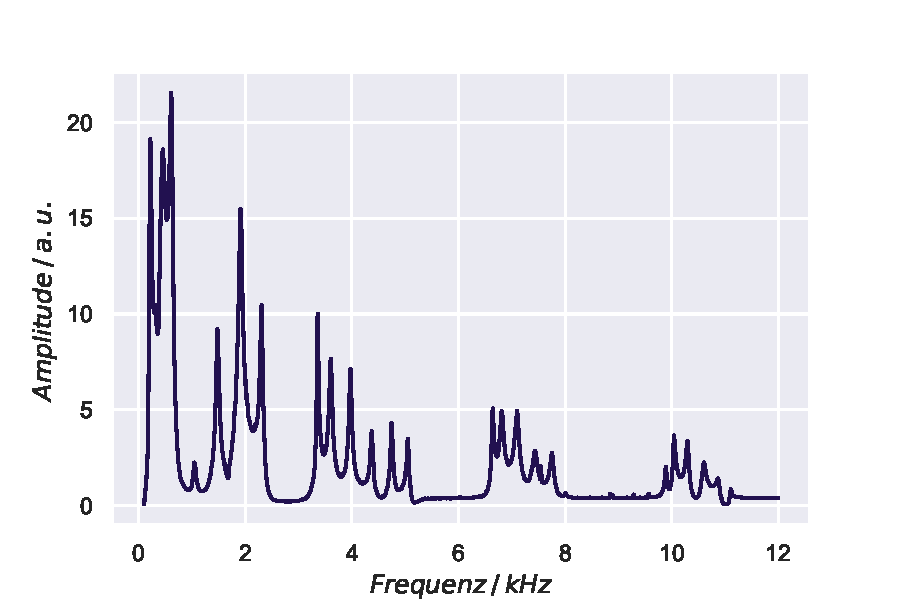
\includegraphics[width=0.5\textwidth]{Daten/Festkörper/FK1_16mm_5.pdf} &   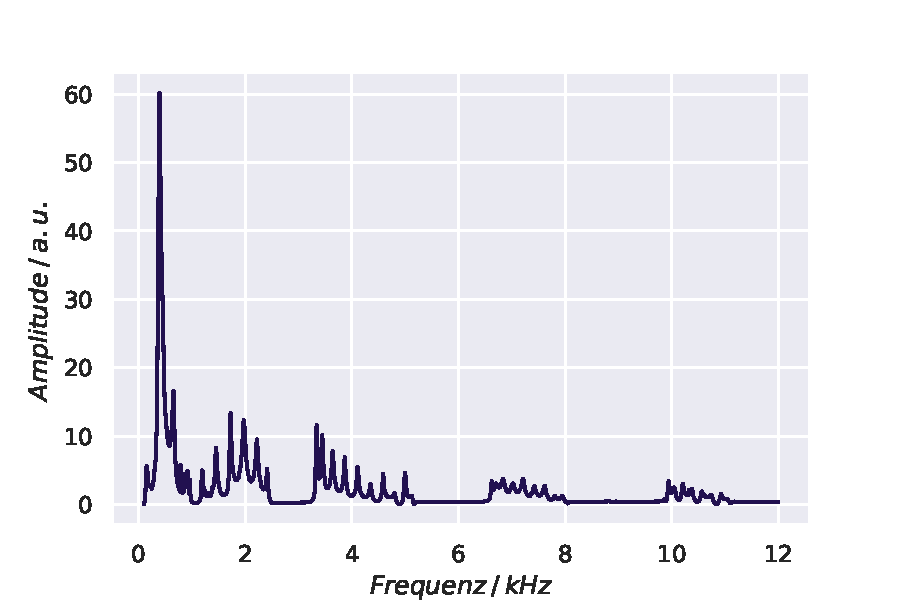
\includegraphics[width=0.5\textwidth]{Daten/Festkörper/FK1_16mm_9.pdf} \\
  (c) 6 Zylinder & (d) 10 Zylinder \\[6pt]
  
  \end{tabular}
  \caption{Die Frequenzspektren der Zylinderketten verschiedener Länge bei einem Irisdurchmesser von $16\, \si{\milli\metre}$} 
  \label{fig:fk1}
\end{figure}
\subsubsection{Blenden verschiedener Durchmesser zwischen den Zylindern in der Resonatorkette}

Das Frequenzspektrum der Resonatorkette mit $2$,$4$ und $10$ Zylindern wurden erneut aufgenommen wobei dieses Mal der Durchmesser der Blenden variiert wurde. 
Die der Vergleich der Frequenzspektren mit verschiedene Blendendurchmesser ist für die Kette aus 10 Zylindern in der Abbildung \ref{fig:fkvergleich} gezeigt. \\
Es ist zunächst zu bemerken, dass die Abstände der Peaks für größere Durchmesser vergrößern. Dies liegt an der veränderten Kopplung zwischen den einzelnen Resonatoren. 
Des Weiteren haben die Peaks der ersten Ordnungen für Blenden mit größerem Durchmesser eine höhere Amplitude. Die somit werden die Peaks erster Ordnungen durch kleinere Blendendurchmesser unterdrückt. 

\begin{figure}[H]
  \centering
  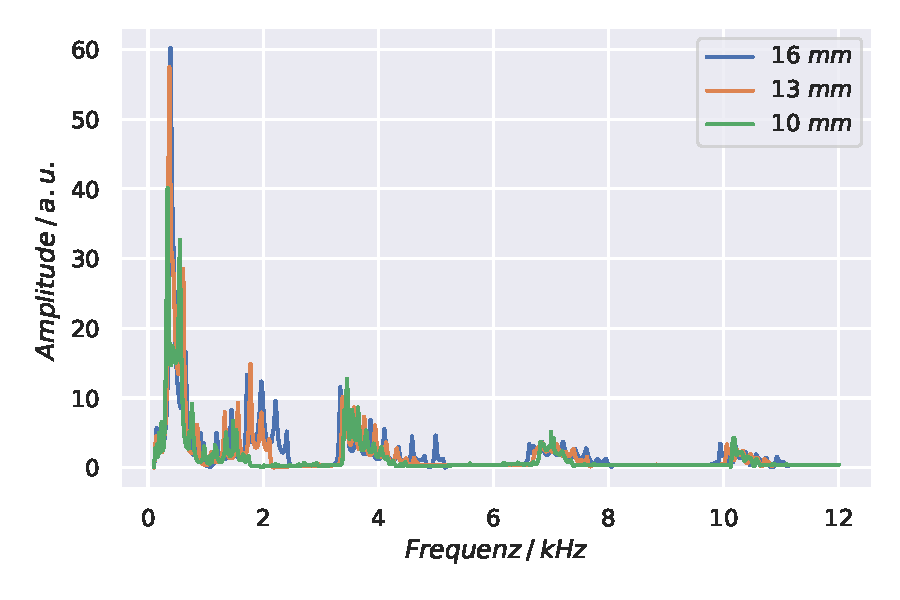
\includegraphics[width=0.8\textwidth]{Daten/Festkörper/vergleich.pdf}
  \caption{Vergleich zwischen den Frequenzspektren der Zylinderketten mit verschiedenen Irisdurchmesser.}
  \label{fig:fkvergleich}
\end{figure}
\subsubsection{Modifikation der Resonatorkette}
\begin{figure}[H]
  \centering
  \begin{tabular}{cc}

  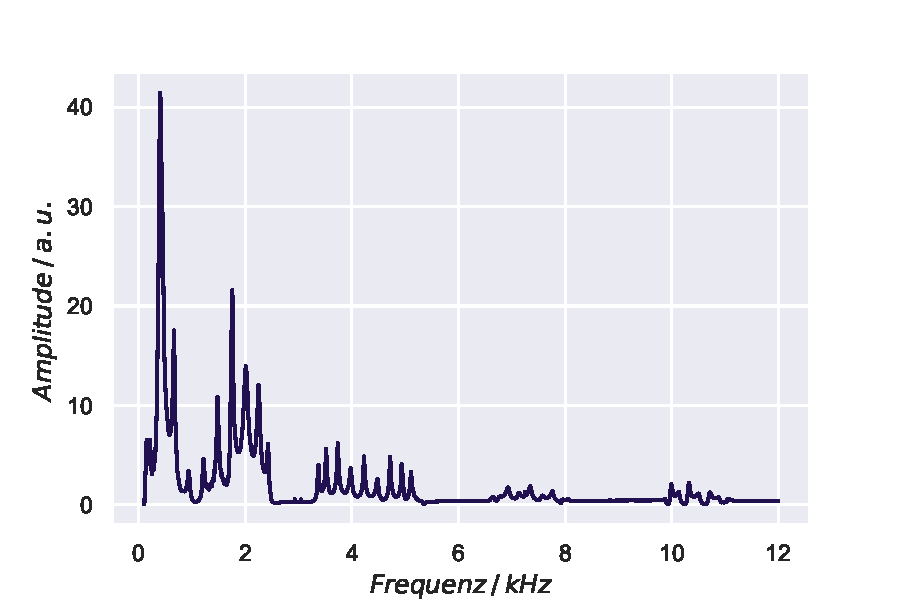
\includegraphics[width=0.5\textwidth]{Daten/Festkörper/FK3_16mm_37-5mm.pdf} &   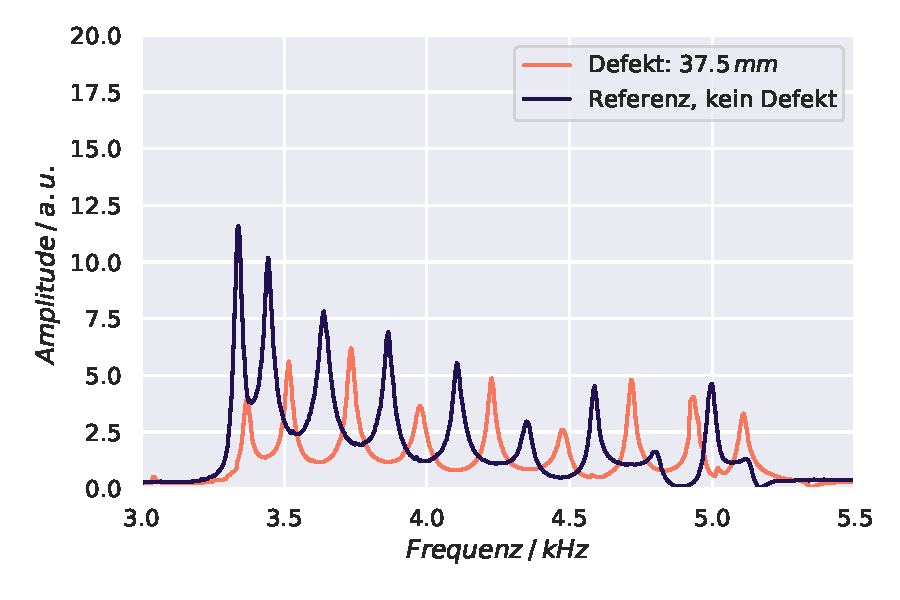
\includegraphics[width=0.5\textwidth]{Daten/Festkörper/FK3_16mm_37-5mmZOOM.pdf} \\
  \multicolumn{2}{c}{(a)  $37.5 \,\si{\milli\metre}$ Zylinder als Defekt}\\[6pt]
  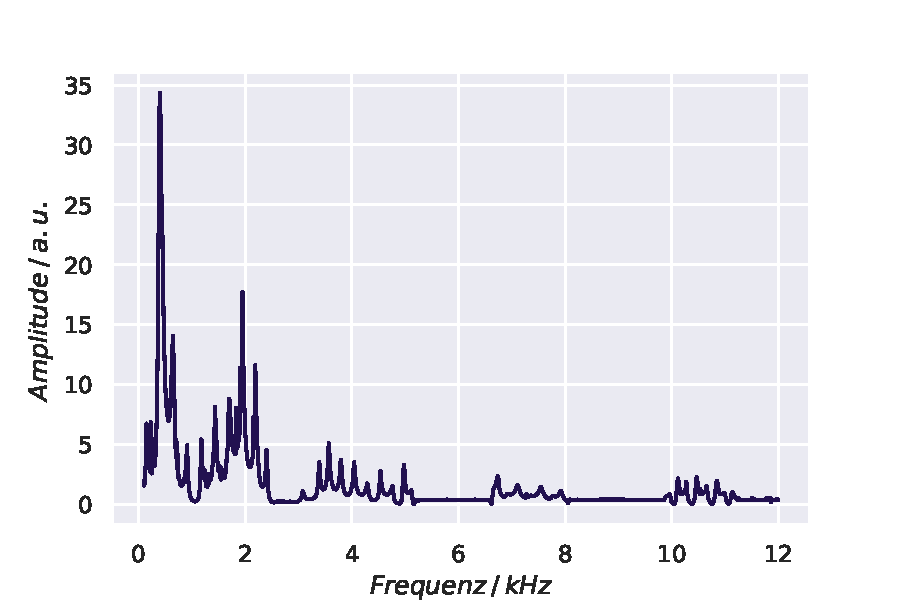
\includegraphics[width=0.5\textwidth]{Daten/Festkörper/FK3_16mm_62-5mm.pdf} &   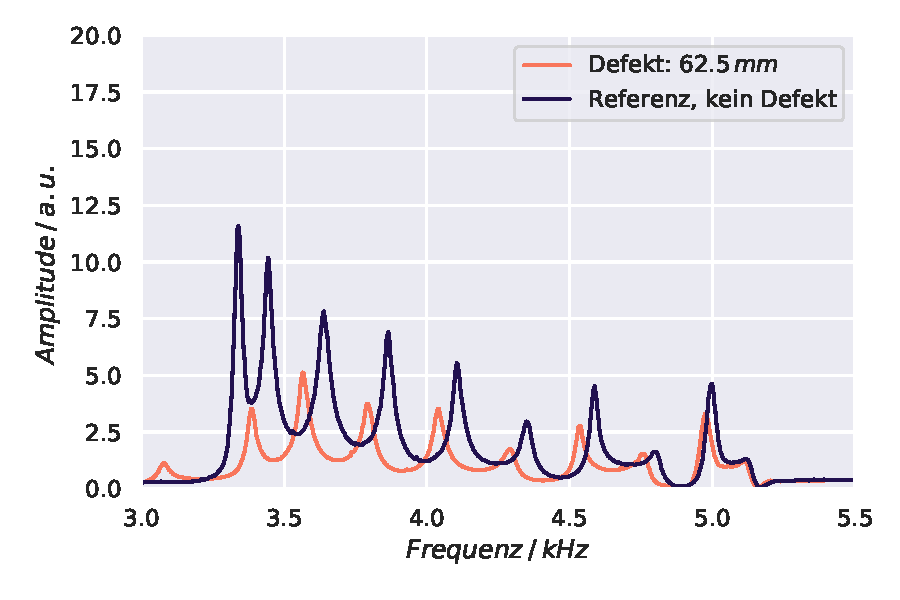
\includegraphics[width=0.5\textwidth]{Daten/Festkörper/FK3_16mm_62-5mmZOOM.pdf} \\
  \multicolumn{2}{c}{(b)  $62.5 \,\si{\milli\metre}$ Zylinder als Defekt}\\[6pt]
  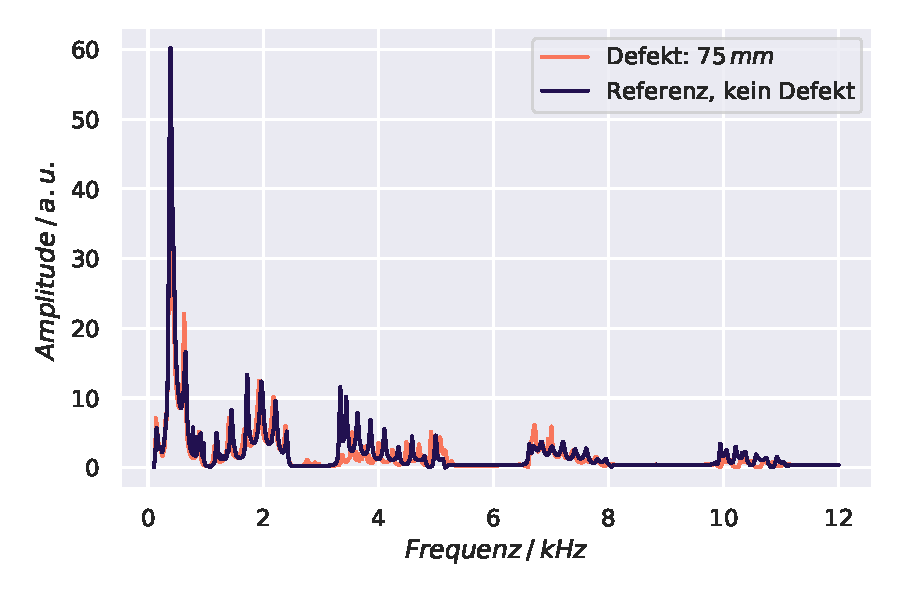
\includegraphics[width=0.5\textwidth]{Daten/Festkörper/FK3_16mm_75mm.pdf} &   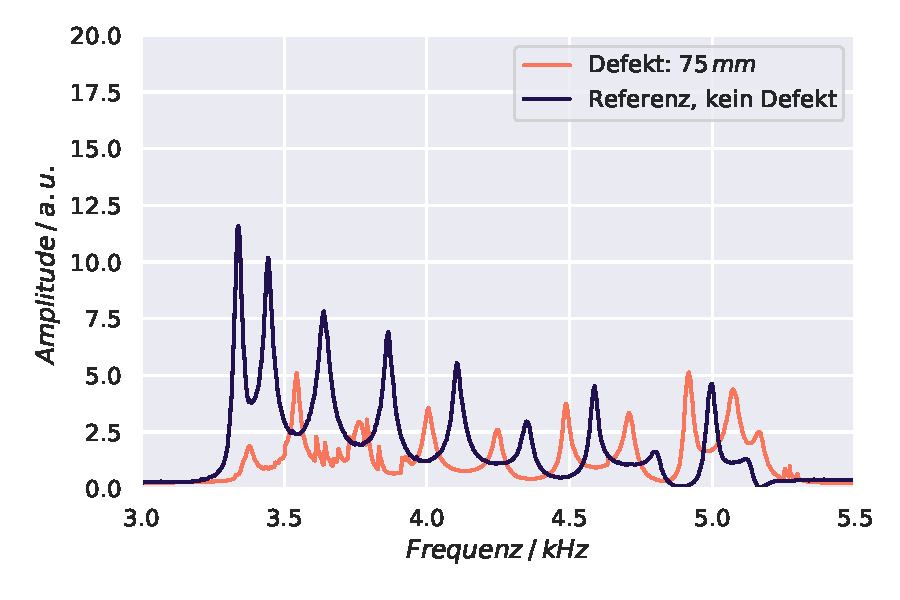
\includegraphics[width=0.5\textwidth]{Daten/Festkörper/FK3_16mm_75mmZOOM.pdf} \\
  \multicolumn{2}{c}{(c)  $75 \,\si{\milli\metre}$ Zylinder als Defekt}\\[6pt]
  
  \end{tabular}
  \caption{Auswirkungen eines Defekts in der Resonatorkette auf das Frequenzspektrum. Die rechten Plots zeigen den Zoom auf das zweite Band.} 
  \label{fig:fkMod}
\end{figure}

\begin{figure}[H]
  \centering
  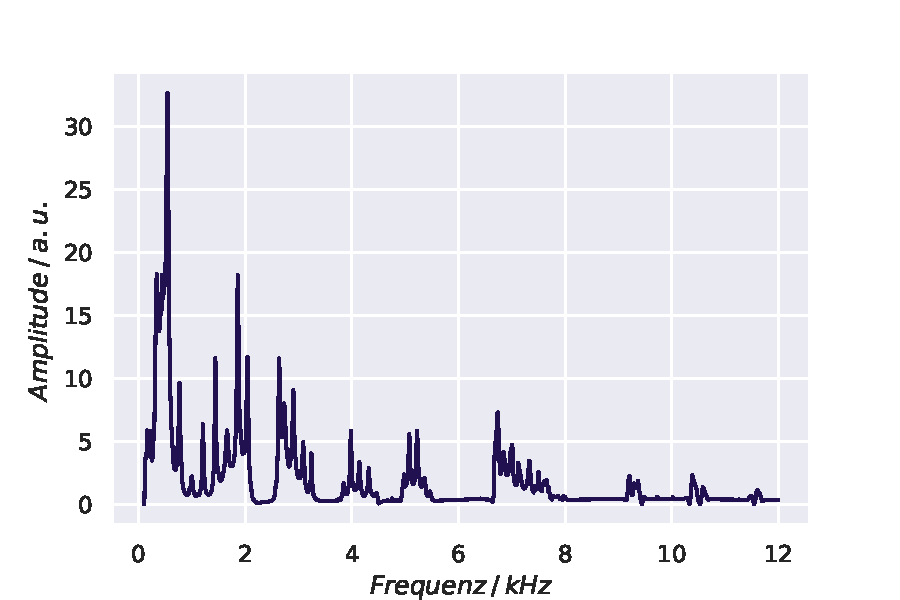
\includegraphics[width=0.7\textwidth]{Daten/Festkörper/FK4.pdf} 
  \caption{Vergleich zwischen dem Frequenzspektrum der Resonatorkette mit abwechselnder Zylinderlänge und dem Spektrum der einzelnen Zylinder.} 
  \label{fig:fkMod2}
\end{figure}